\documentclass[sigconf]{acmart}




\usepackage{color}
\usepackage{listings}
\usepackage{amsmath}


\newcommand{\nats}{\ensuremath{\mathbb{N}}}

\lstset{
  language=haskell,
  basicstyle=\footnotesize\ttfamily,breaklines=true,
  frame=none,
  literate=
    {->}{{$\rightarrow\;$}}1
    {=>}{{$\Rightarrow\;$}}1
    {++}{{\code{++}}}1
    {~}{{\ }}1
    {\\dollar}{{$\$$\;}}1,
  % Style for (listings') identifiers
  identifierstyle={\ttfamily\color{black}},
  % Style for declaration keywords
  keywordstyle=[1]{\ttfamily\color{violet}},
  % Style for gallina keywords
  keywordstyle=[2]{\ttfamily\color{green}},
  % Style for sorts keywords
  keywordstyle=[3]{\ttfamily\color{blue}},
  % Style for tactics keywords
  keywordstyle=[4]{\ttfamily\color{blue}},
  % Style for terminators keywords
  keywordstyle=[5]{\ttfamily\color{red}},
  morekeywords=[1]{class, instance},
  morekeywords=[2]{where},
  morekeywords=[3]{Maybe},
  morekeywords=[4]{main},
  morekeywords=[6]{do, proc, last, first, try, idtac, repeat},
}



% Copyright
%\setcopyright{none}
%\setcopyright{acmcopyright}
%\setcopyright{acmlicensed}
\setcopyright{rightsretained}
%\setcopyright{usgov}
%\setcopyright{usgovmixed}
%\setcopyright{cagov}
%\setcopyright{cagovmixed}


% DOI
\acmDOI{10.475/123_4}

% ISBN
\acmISBN{123-4567-24-567/08/06}

%Conference
\acmConference[SCAV]{ACM}{2017}{USA} 
\acmYear{2017}
\copyrightyear{2017}

\acmPrice{15.00}


\begin{document}
\title{Using Functional Reactive Programming to Build Safer Autonomous Vehicle Controllers}
\subtitle{An opensource tool}

\author{Bernd Finkbeiner}
\orcid{1234-5678-9012}
\affiliation{%
  \institution{University of Saarland}
  \state{Germany} 
}

\author{Felix Klein}
\orcid{1234-5678-9012}
\affiliation{%
  \institution{University of Saarland}
  \state{Germany} 
}

\author{Ruzica Piskac}
\orcid{1234-5678-9012}
\affiliation{%
  \institution{Yale University}
  %\streetaddress{}
  \state{CT, USA} 
}

\author{Mark Santolucito}
\orcid{1234-5678-9012}
\affiliation{%
  \institution{Yale University}
  %\streetaddress{}
  \state{CT, USA} 
}

\begin{abstract}
Functional languages have provided major benefits to the verification community.
Although features such as purity, a strong type system, and computational abstractions can help guide programmers away from costly errors, these can present challenges when used in a reactive system.
Functional Reactive Programming is a paradigm that allows users the benefits of functional languages and an easy interface to a reactive environment.
We present a tool for building autonomous vehicle controllers in FRP using Haskell.
\end{abstract}

%
% The code below should be generated by the tool at
% http://dl.acm.org/ccs.cfm
% Please copy and paste the code instead of the example below. 
%
\begin{CCSXML}
<ccs2012>
 <concept>
  <concept_id>10010520.10010553.10010562</concept_id>
  <concept_desc>Computer systems organization~Embedded systems</concept_desc>
  <concept_significance>500</concept_significance>
 </concept>
 <concept>
  <concept_id>10010520.10010575.10010755</concept_id>
  <concept_desc>Computer systems organization~Redundancy</concept_desc>
  <concept_significance>300</concept_significance>
 </concept>
 <concept>
  <concept_id>10010520.10010553.10010554</concept_id>
  <concept_desc>Computer systems organization~Robotics</concept_desc>
  <concept_significance>100</concept_significance>
 </concept>
 <concept>
  <concept_id>10003033.10003083.10003095</concept_id>
  <concept_desc>Networks~Network reliability</concept_desc>
  <concept_significance>100</concept_significance>
 </concept>
</ccs2012>  
\end{CCSXML}

\ccsdesc[500]{Computer systems organization~Embedded systems}
\ccsdesc[300]{Computer systems organization~Redundancy}
\ccsdesc{Computer systems organization~Robotics}
\ccsdesc[100]{Networks~Network reliability}

% We no longer use \terms command
%\terms{Theory}

\keywords{FRP, Autonomous Vehicles}


\maketitle

\section{Introduction}

Autonomous vehicles are considered to be one of the most challenging
types of reactive systems currently under development~\cite{AlurMT16,
  WongpiromsarnKF11, RamanDSMS15}. They need to interact reliably with
a highly reactive environment and crashes cannot be tolerated.  Life
critical decisions have to be made instantaneously and need to be
executed at the right point in time.

The development of autonomous vehicles and other cyberphysical systems
is supported by a wide spectrum of
programming and modelling methodologies, 
including synchronous programming languages like Lustre~\cite{conf/popl/CaspiPHP87} 
and Esterelle~\cite{conf/concur/BerryC84},
hardware-oriented versions of imperative programming languages like
SystemC~\cite{open2006ieee}, and visual languages like MSCs and Stateflow-charts~\cite{harel2003message,journals/scp/Harel87}.
The question of which programming paradigm is best-suited to write
easy-to-understand, bug-free code is still largely unresolved.

In the development of other forms of critical software, outside the
embedded domain, developers increasingly turn to functional
programming (cf.~\cite{frankau2009commercial}).  The strong type system in functional
languages largely eliminates runtime errors~\cite{cardelli1996type}.
Higher-order functions like \texttt{map} often eliminate the need for
explicit index counters, and, hence, the risk of ``index out of
bounds'' errors.  Functional purity reduces the possibility of
malformed state that can cause unexpected behavior.

While mathematical models of embedded and cyberphysical systems often
rely on functional notions such as stream-processing
functions~\cite{DBLP:series/mcs/BroyS01,DBLP:conf/csdm/Broy12}, the
application of functional programming in the practical development of
such systems has, so far, been limited. One of the most advanced
programming language in this direction is Ivory, which was used in the
development autonomous vehicles~\cite{pike2014}.  Ivory is a
restricted version of the C programming language, embedded in Haskell.
It provides access to the low level operations necessary for embedded
system programming, but still enforces good programming practice, such
as disallowing pointer arithmetic, with a rich type system.

Ivory does not, however, have an explicit notion of time.
It cannot then deal directly with the integration of 
continuous and discrete time, which is fundamental for the
development of a cyberphysical system. For example,
in a car, continuous signals, such as the velocity or acceleration,
mix with the discrete steps of the digital controller.

In this paper, we investigate the use of functional programming
in a domain where the interaction between continuous and discrete signals
is of fundamental importance. We build a vehicle controller capable
of both autonomous vehicle control and multi-vehicle communication,
such as the coordination in platooning situations.

Our approach is based on Functional Reactive Programming
(FRP)~\cite{hudak2003arrows,hudak2000haskell}.
The fundamental idea of FRP is to extend the classic building blocks 
of functional programming (\eg monads, arrows,
applicatives)
with the abstraction of a \emph{signal} to
describe time-varying values. FRP programs can be exceptionally
efficient.  For example, a network controller recently implemented as
an FRP program on a multicore processor outperforms any other such
controller existing today~\cite{Voellmy:2012:SSD:2377677.2377735}.

We have built a library, \ourLib, to use FRP to control a vehicle inside a simulation.
The library interfaces Haskell FRP programs to TORCS, The Open Racing Car Simulator, an open-source vehicle simulator~\cite{torcs}.
TORCS has been used in the Simulated Car Racing Championship competition~\cite{SCRC}, as well as other autonomous vehicle research projects~\cite{xu2016experimental,OnievaPAMP09,conf/cig/CardamoneLL09,conf/cig/MunozGS10}. 
Through \ourLib, the Haskell program has access to the sensors and actuators of the car, as well
as the communication channels between different vehicles.
Such a simulator is a  critical component of modern autonomous vehicle research, especially towards the goal of safe platooning algorithms~\cite{kamali2016formal}.

We report on experience with a case study, in which we implement a controller for a car on an empty race trace. 
Our controller successfully navigates the TORCS preloaded tracks with a reasonable speed and finesse, similar to that expected of an average driver (see Fig.~\ref{fig:race}). 
Furthermore, the case study illustrates that the functional approach indeed leads to elegant, easily understandable, and safe code.

\begin{figure}[t]
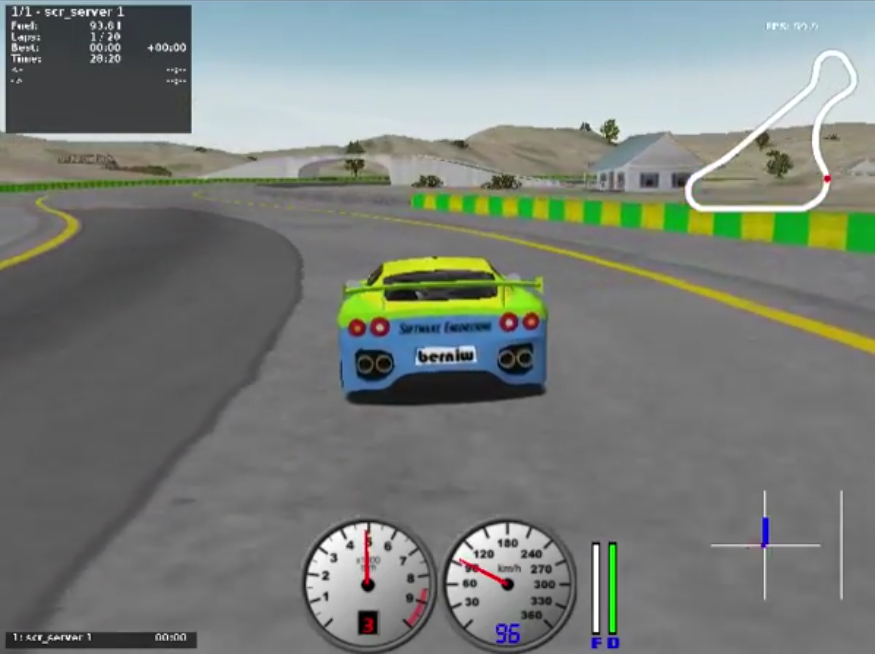
\includegraphics[width=0.45\textwidth]{figs/racing.png}
\caption{A screenshot of Haskell controlling the autonomous vehicle in the TORCS simulator}
\label{fig:race}
\end{figure}

\section{FRP}

\subsection{Preliminaries}

One of the classic approaches to build reactive systems is to use a call-back framework, that can be embedded inside a loop.
The call-back can be used to query the state of value, or to change that value.
With FRP, we instead introduce an abstractions of time that allow the programmer to directly manipulate some time-varying value.
This key abstraction is called a \textit{signal}, and has the following type:

\begin{lstlisting}
type Signal a = Time -> a
\end{lstlisting}

A signal is then a function that relates time to some value.
For example, the type \texttt{Signal Image} would then be video data, and \texttt{Signal Steer} would be the way a steering wheel is operated over time.
With signals, FRP also introduces the abstraction of a \textit{signal function (SF)}.
This is a transformer from one signal to another.

\begin{lstlisting}
type SF a b = Signal a -> Signal b
\end{lstlisting}

Using the previous signals, we can then introduce a type for a steering function that operates based on a video stream as \texttt{turn :: SF Image Steer}.
This function will process video and use it to decide how to steer.
We omit an implementation, as the details of the data transformation are not relevant to the structure of the FRP code.

There are many types of FRP based on different abstractions.
The monad abstraction can be used to handle signal processing~\cite{van2014monadic},
 but we will instead choose to focus on a FRP library, Yampa, that uses the arrow abstraction~\cite{hudak2003arrows}, so called Arrowized FRP.
Arrow generally run faster with little need for manual optimization~\cite{yallop2016causal}, but are fundamentally less expressive than a monadic FRP~\cite{lindley2011idioms}.
This can be beneficial because the more restrictive our languages, the less likely it is for a programmer to make a mistake.
As we will see in the sequel, Yampa is still powerful enough to write a controller to drive an autonomous vehicle.
At the same time, the style is also syntactically clear accessible to make for an easy introduction to the FRP paradigm.

In Arrowized FRP, Haskell provides an special syntax.
This is a composition environment, in which the programmer only manages the composition of arrow functions.
Inputs are read in from the right hand side, and piped to the left hand side.
This is demonstrated in Listing~\ref{lst:arrows}.

\begin{lstlisting}[float,floatplacement=h!,caption=Basic Arrowized FRP syntax,label=lst:arrows]
myDriver :: SF Image Steer
myDriver = proc image -> do
  basicSteer    <-     turn  -< image
  adjustedSteer <- arr avoid -< (image,basicSteer)
  returnA -< adjustedSteer
\end{lstlisting}

In this example, we introduce \texttt{avoid :: (Image,Steer) -> Steer}, a new function that will adjust our basic steering plan based on the image to avoid any obstacles.
In the above example, this function is lifted to the signal level using \texttt{arr :: (a -> b) -> SF a b}.
Since \texttt{turn} was already on the signal level, we did not need to apply the lifting function.

We can also imagine that our function to avoid obstacles requires two images to calculate the adjusted steering command.
This might be to filter noise in the image, or to calculate the velocity of an approaching obstacle.
In this case, we will need to save the previous state of the image for the next processing turn.
This can be achieved by using an ArrowLoop instance with the \texttt{rec} keyword.
Eliding the technical details for the purposes of this presentation, the syntax looks as shown in Listing~\ref{lst:loop}.

\begin{lstlisting}[float,caption=Using ArrowLoop to send feedback,label=lst:loop]
myDriver :: SF Image Steer
myDriver = proc image -> do
  rec
    oldI          <- iPre null -< image
    basicSteer    <-     turn  -< image
    adjustedSteer <- arr avoid -< (image,oldI,basicSteer)
  returnA -< adjustedSteer
\end{lstlisting}

The function \texttt{iPre} will take some initial state, in this case a null image, and save images for one time step each time it is processed.
This creates a type of feedback loop that is then used in the updated \texttt{avoid} function.
The \texttt{rec} keyword is used to denote a section of arrow code that has a mutual dependency.
Without the keyword, there would be an unresolvable dependency loop in the code.




\subsection{Case Study : Driving}
A driver observes the environment and changes the drive state over time.
This is represented as a \textit{signal function (SF)} in Yampa.

\begin{lstlisting}
type Driver = SF CarState DriveState
\end{lstlisting}

We then can create a driver as shown in Listing~\ref{lst:driver}
This is the entirety of the code needed for a basic controller that can successfully, and with some speed and finesse, navigate a vehicle in track shown in Fig.~\ref{fig:race}.

One major advantage of FRP is separation of control flow and data level manipulation. 
This abstraction makes it possible to easily reason about each of the components without worrying about confounding factors from the other.
For example, the user may only be concerned with verifying that their steering control is correct.
The user then only needs to verify the \texttt{steering} function in isolation from all other code.
This is a pure function, as evidenced by the type signature, which produces a new steering value based on the angle relative to the edges of the track and position on the track (where 0 is centered between the edges, and 1 is the left wall).

%\begin{minipage}{\linewidth}
\begin{lstlisting}[float,floatplacement=TR,caption=A complete basic controller in Yampa, label=lst:driver]
myDriver :: Driver
myDriver = proc CarState{..} -> do
  rec 
    oldG <- iPre 0 -< g
    g <- arr shifting -< (rpm,oldG)
    s <- arr steering -< (angle,trackPos)
    a <- arr gas -< (speedX,s)
  returnA -< defaultDriveState {accel = a, gear = g, steer = s}

shifting :: Double -> Int
shifting (rpm,g) = if 
  | rpm > 6000 -> min 6 (g+1)
  | rpm < 2000 -> max 1 (g-1)
  | otherwise  -> g
 
steering :: (Double,Double) -> Double
steering (spd,trackPos) = let
  turns = spd*14 / pi
  centering = turns - (trackPos*0.1)
  clip x = max (-1) (min x 1)
 in
  clip centering
  
targetSpeed = 100
gas :: (Double,Double) -> Double
gas (speed,steer) = 
  if speed < (targetSpeed-(steer*50)) then 1 else 0
\end{lstlisting}
%\end{minipage}


\section{\ourLib}

\subsection{Basics}

We have developed a library for programming controllers for autonomous vehicles using FRP, and connecting those controllers to the TORCS vehicle simulator.
This library, \ourLib, uses Yampa as the core FRP library, though the structure can easily be adapted to any Haskell FRP library.

The core functionality of \ourLib is captured in the function \texttt{startDriver :: Driver -> IO()}.
This function will automatically connect a controller, expressed with the \texttt{Driver} type, to TORCS, which results in continuous \texttt{IO()} actions.
The user must implement a controller that will process all the data available from the sensors \texttt{CarState}, and output a commands to the vehicle, as a \texttt{DriveState}.

\begin{lstlisting}
type Driver = SF CarState DriveState
\end{lstlisting}

\subsection{Case Study : Driving}

As a demonstration of the \ourLib library in use, we present a case study on a simple controller for a car on an empty race track.
We implement a controller in FRP using Yampa, as shown in Listing~\ref{lst:driver}, that can be connected to TORCS using our library, \ourLib.
This code is complete and can be run as-is with an installation of TORCS.
This controller can successfully, and with some speed and finesse, navigate a vehicle in track shown in Fig.~\ref{fig:race}.

Our controller uses ArrowLoop to keep track of the current gear of the car.
Although the gear is available as sensor data, it is illustrative to keep track locally of this state.
In general, the ArrowLoop can be used to maintain any state that may be of interest in a future processing step.
Additionally, notice all of the data manipulation functions are pure, and lifted via \texttt{arr}.
One major advantage of FRP is this separation of dependency flow and data level manipulation. 

This abstraction makes it possible to easily reason about each of the components without worrying about confounding factors from the other.
For example, if a programmer wants to verify that the steering control is correct, it is semantically guaranteed that the only function that must be checked is \texttt{steering}.
Because of Haskell's purity, this is the only place where the steering value may be changed, significantly reducing the size of the verification problem.

\begin{lstlisting}[float,floatplacement=TR,caption=A complete basic controller in Yampa, label=lst:driver]
{-# LANGUAGE Arrows,
             MultiWayIf,
             RecordWildCards #-}
module TORCS.Example where
import TORCS.Connect
import TORCS.Types

main = startDriver myDriver

myDriver :: Driver
myDriver = proc CarState{..}  -> do
  rec 
    oldG <- iPre 0 -< g
    g <- arr shifting -< (rpm,oldG)
    s <- arr steering -< (angle,trackPos)
    a <- arr gas -< (speedX,s)
  returnA -< defaultDriveState {accel = a, gear = g, steer = s}

shifting :: (Double,Int) -> Int
shifting (rpm,g) = if 
  | rpm > 6000 -> min 6 (g+1)
  | rpm < 2000 -> max 1 (g-1)
  | otherwise  -> g
 
steering :: (Double,Double) -> Double
steering (spd,trackPos) = let
  turns = spd*14 / pi
  centering = turns - (trackPos*0.1)
  clip x = max (-1) (min x 1)
 in
  clip centering

targetSpeed = 100
gas :: (Double,Double) -> Double
gas (speed,steer) = 
  if speed < (targetSpeed-(steer*50)) then 1 else 0
\end{lstlisting}


\subsection{Multi-Vehicle Communication}

Thanks to functional language's exceptional support for parallelism, controlling multiple vehicles in a multi-threaded environment is exceedingly simple. 
In our library API, the user simply needs to use \texttt{startDrivers} rather than \texttt{startDriver}, and pass a list of \texttt{Driver} signal function that should drive together.
This can be used to race various implementations against each other, or it can be used to build a vehicle platooning controller.
In this case, the user will need to be able to simulate communication between the vehicles.

Our library provides a simple interface for simulating communication between vehicles.
In order to broadcast a message to the other vehicles in the simulation, the controller simply writes a message to the \texttt{broadcast} field of the output \texttt{DriveState}.
That message is then broadcast to all other vehicles as soon as possible, and received in the \texttt{communication} field of the input \texttt{CarState}.

We allow all vehicles in the simulation to communicate irrespective of distance and with zero packet loss.
If a user wishes to simulate unreliable communications, or distance constraints, this can be simulated on a case-by-case basis.

\section{Implementation}

The Open Racing Car Simulator (TORCS) is an existing open source vehicle simulatori~\cite{torcs}.
It has been used in the Simulated Car Racing Championship competition~\cite{SCRC}.
For these competitions, a car can be controller via a socket that sends the sensor data from the vehicle and can receive and process the driving commands.

We implemented an open source library for interfacing Haskell FRP programs to TORCS.
The library is available at \url{https://github.com/santolucito/Haskell-TORCS}.

While there are existing bindings to these socket protocols for languages such as python~\cite{snakeoil,pyscrc}, we are the first such binding for Haskell.
This is likely due in part to the unique style of programming that is required for streaming socket programming in Haskell due to its purity.
With the assistance of FRP, we solved this problem in a principled way that allows users to manipulated sensor data in a transparent and structured way.


Although the existing tool is specifically tailored to be used with our controller using the Yampa library,
  minor modifications can allow the tool to easily work with other FRP libraries.

It may also be interesting to build more lower level binding to allow non-FRP Haskell program to interface with TORCS.
While FRP is one of the simplest interfaces for reactive systems programming in functional languages, it is also possible to use functional language in this context without FRP.


\section{Related Work}

TORCS has been used as a simulator for formal verification of platoons~\cite{kamali2016formal}, etc... \cmark{TODO pick a few TORCS paper from google scholar}.
None of these works have used FRP as the language for the controller.


FRP specifically has been proposed as a tool for vehicle control~\cite{kazemi2016,zou2016}.
This work extends FRP to also prioritize certain functions for timing constraints.
This has been not yet been tested on vehicle simulation, in part due to the lack of a simulator compatible with the FRP language model.

FRP has been used for embedded systems~\cite{helbling2016juniper} and networking~\cite{voellmy2012scalable}.
The FRP networking library took advantage of Haskell's multicore support and significantly outperformed competing tools written in C++ and Java.


To the best of our knowledge this is the first FRP-based vehicle simulator.
Although there are many bindings to various vehicle simulators, these tend to use imperative languages.
For instance, TORCS allows users to directly edit the source code and add a new car in C++.
There are also TORCS bindings for python, java, and matlab, which have been used in the SCRC competition~\cite{SCRC}.

The videogame GTA~\cite{} has also been used to train image recognition software for autonomous vehicles~\cite{}.
While GTA is professionally produced game, which has more attractive graphics and a more advanced physics engine, it has a different set of issues.
First, is that as proprietary software that was not designed for autonomous vehcile reserach, the ability to build sensor based controllers is more restricted. 
Furthermore, unlike TORCS, which is designed primarily as a vehicle simulator, GTA's physics engine is tuned to maximize entertainment.
Using GTA as a meaningful control simulator would still be valuable work, but we leave this to future explorations.

\section{Future Work}

Although FRP supports both handling of continuous and discrete behaviors, we have treated all data as continuous.
For example, we have chosen to implement the communications protocol as continuous, though it would be interesting to explore the implications of a discrete model
Additionally, FRP may particularly well-suited to be used in a human-in-the-loop setting, where discrete user actions must be considered in addition to sensor data.



\bibliographystyle{ACM-Reference-Format}
\bibliography{sigproc} 

\end{document}
